\documentclass{article}
\usepackage[utf8]{inputenc}
\usepackage[english]{babel}
\usepackage[font=small,labelfont=bf]{caption}
\usepackage{geometry}
\usepackage{natbib}
\usepackage{pxfonts}
\usepackage{graphicx}
\usepackage{newfloat}
\usepackage{setspace}
\usepackage{hyperref}
\usepackage{placeins}
\usepackage{rotating}

\newcommand{\argmax}{\mathop{\mathrm{argmax}}\limits}
\newcommand{\argmin}{\mathop{\mathrm{argmin}}\limits}

\newcommand{\demo}{1}

\title{\textit{Supplementary materials for}: Carryover effects in free recall reveal how prior experiences influence memories of new experiences}
\author{Jeremy R. Manning\textsuperscript{1, *}, Andrew C. Heusser\textsuperscript{1, 2}, Kirsten Ziman\textsuperscript{1, 3},\\Emily Whitaker\textsuperscript{1}, and Paxton C. Fitzpatrick\textsuperscript{1}\\\textsuperscript{1}Dartmouth College\\\textsuperscript{2}Akili Interactive\\\textsuperscript{3}Princeton University\\\textsuperscript{*}Corresponding author: jeremy.r.manning@dartmouth.edu}
\date{}

\begin{document}

\renewcommand{\figurename}{Supplementary Figure}

%\begin{titlepage}
%  \maketitle
%  \thispagestyle{empty}
%\end{titlepage}

\setcounter{equation}{0}
\setcounter{figure}{0}
\setcounter{table}{0}
\setcounter{page}{1}
\setcounter{section}{0}
\makeatletter
\renewcommand{\theequation}{S\arabic{equation}}
\renewcommand{\thefigure}{S\arabic{figure}}
\renewcommand{\bibnumfmt}[1]{[S#1]}
\renewcommand{\citenumfont}[1]{S#1}

\maketitle

\begin{figure}[p] \centering
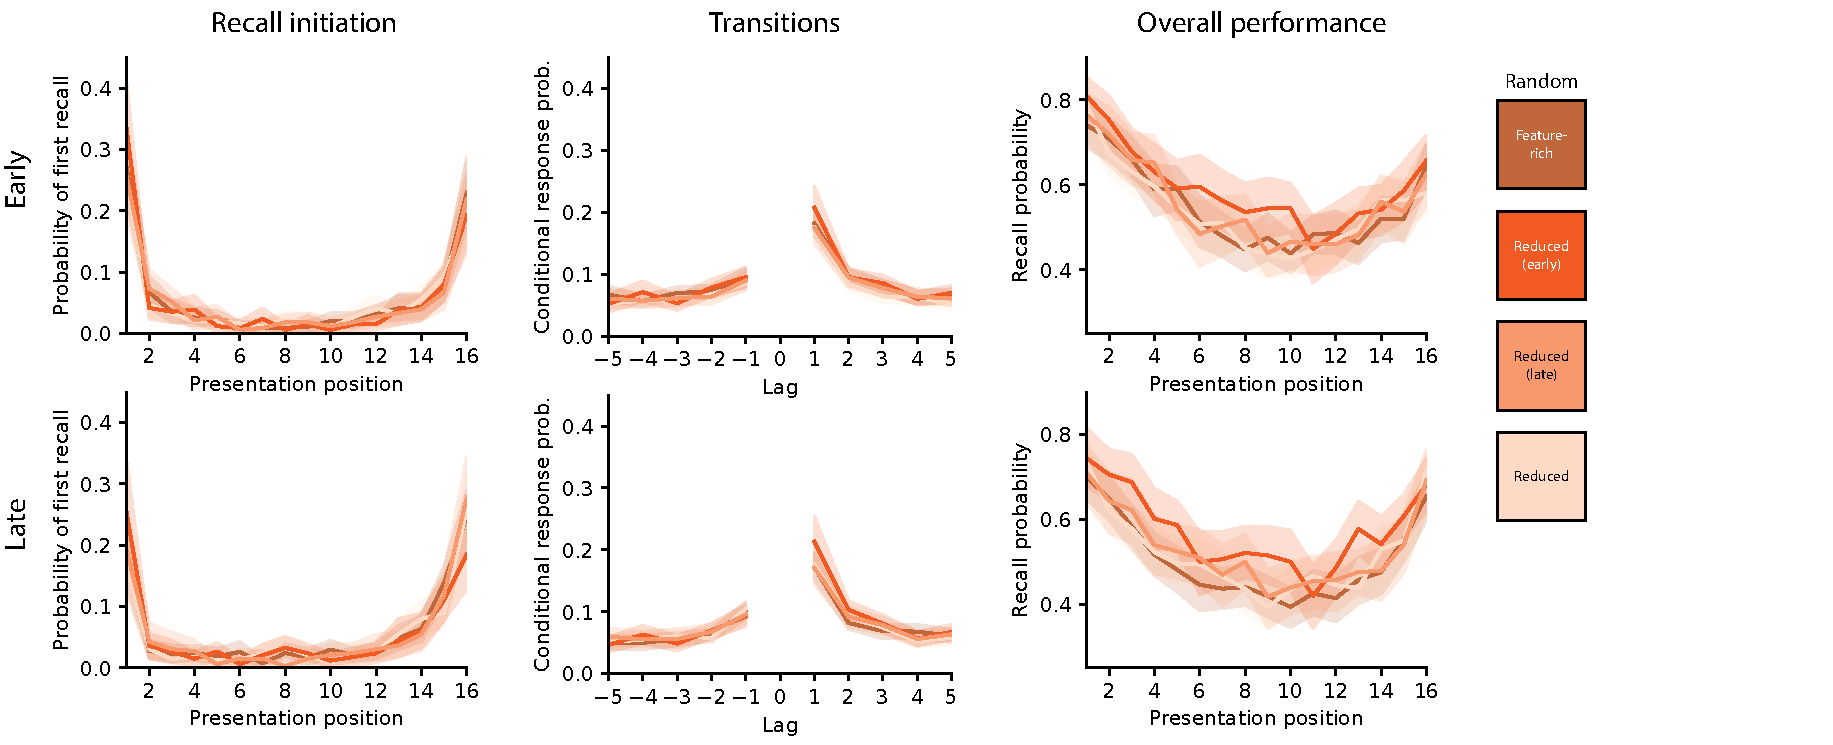
\includegraphics[width=\textwidth]{figures/recall_dynamics_random}

\caption{\textbf{Recall dynamics in feature rich free recall (random conditions).} \textbf{Left panels.} The probabilities of
initiating recall with each word are plotted as a function of presentation
position. \textbf{Middle panels.} The conditional probabilities of recalling
each word are plotted as a function of the relative position (Lag) to the words
recalled just-prior. \textbf{Right panels.} The overall probabilities of
recalling each word are plotted as a function of presentation position.
\textbf{All panels.} Error ribbons denote bootstrap-estimated 95\% confidence
intervals (calculated across participants). Top panels display the recall
dynamics for early (order manipulation) lists in each condition (color). Bottom
panels display the recall dynamics for late (randomly ordered) lists.}

    \label{fig:recall-dynamics-random}
\end{figure}

\begin{figure}[p] \centering
    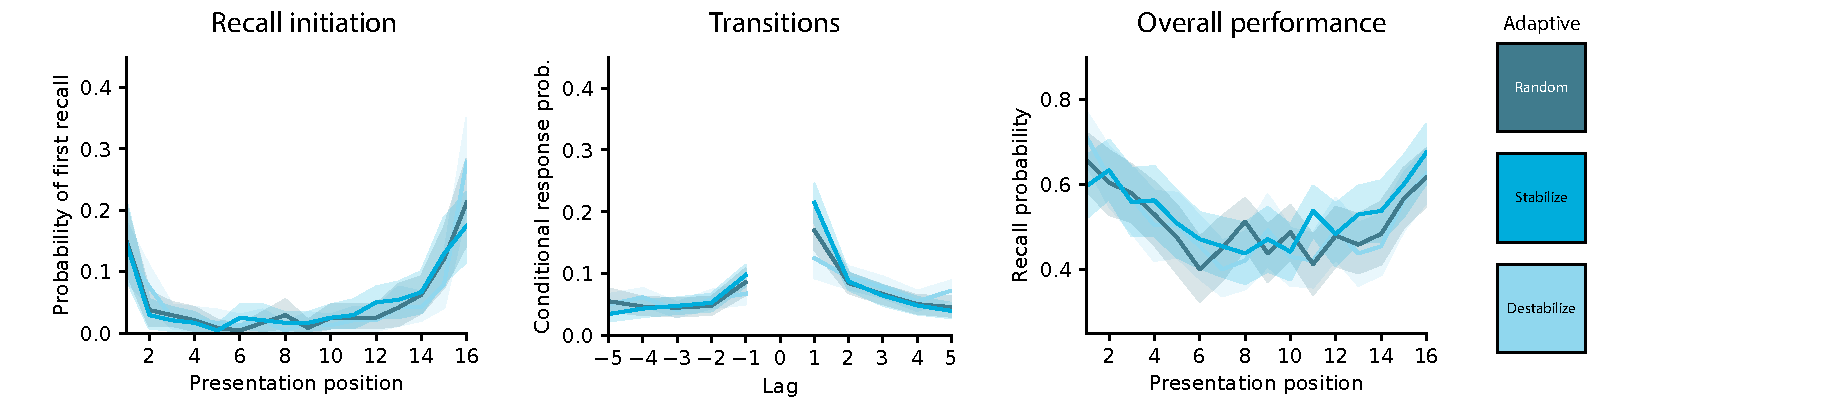
\includegraphics[width=\textwidth]{figures/recall_dynamics_adaptive}
    
    \caption{\textbf{Recall dynamics in feature rich free recall (adaptive conditions).} \textbf{Left panels.} The probabilities of
    initiating recall with each word are plotted as a function of presentation
    position. \textbf{Middle panels.} The conditional probabilities of recalling
    each word are plotted as a function of the relative position (Lag) to the words
    recalled just-prior. \textbf{Right panels.} The overall probabilities of
    recalling each word are plotted as a function of presentation position.
    \textbf{All panels.} Error ribbons denote bootstrap-estimated 95\% confidence
    intervals (calculated across participants). Condition is denoted by color.}
    
        \label{fig:recall-dynamics-adaptive}
    \end{figure}

\begin{figure}[tp] \centering
    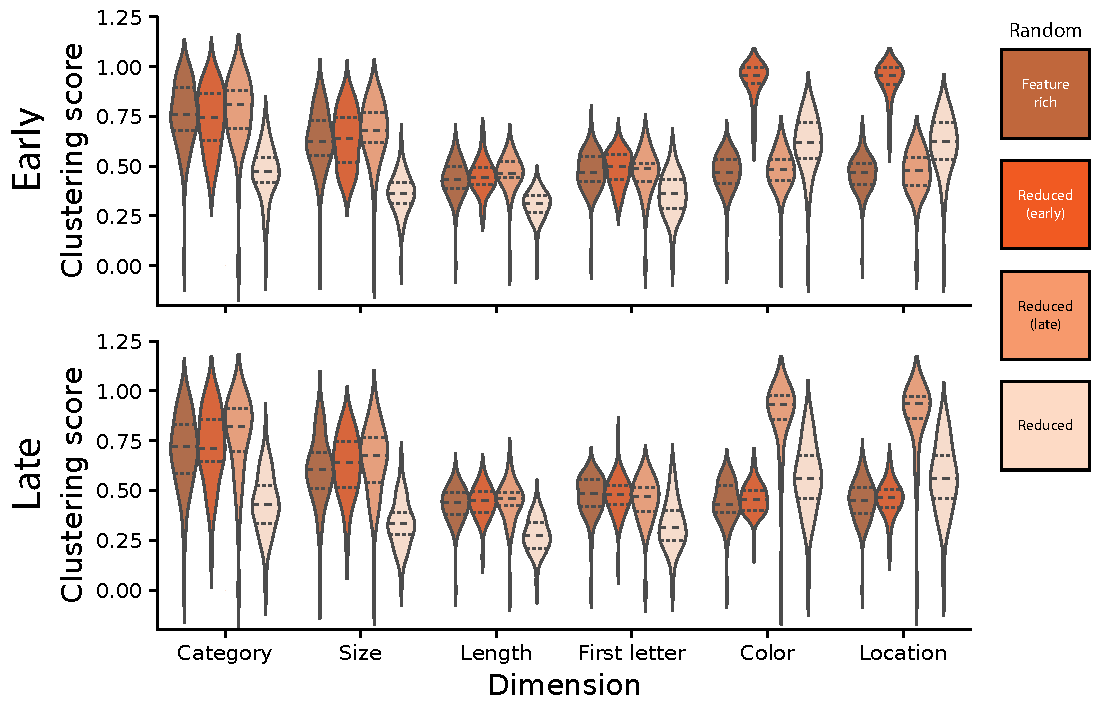
\includegraphics[width=\textwidth]{figures/fingerprints_random}
    
    \caption{\textbf{Memory ``fingerprints'' (random conditions).}
    The across-participant distributions of clustering scores for each feature
    type ($x$-coordinate) are displayed for each experimental condition
    (color), separately for early (top) and late (bottom) lists.}
        \label{fig:fingerprints-random}
\end{figure}
    
\begin{figure}[tp] \centering
    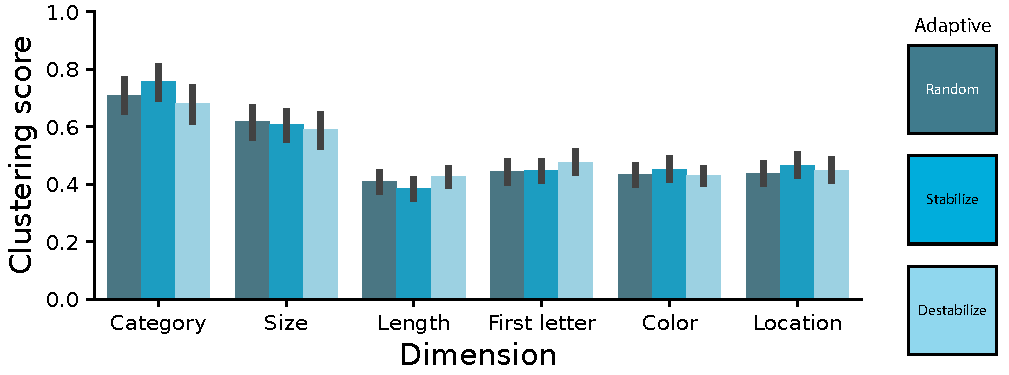
\includegraphics[width=\textwidth]{figures/fingerprints_adaptive}
    
    \caption{\textbf{Memory ``fingerprints'' (adaptive conditions).}
    The across-participant distributions of clustering scores for each feature
    type ($x$-coordinate) are displayed for each experimental condition
    (color).}
        \label{fig:fingerprints-adaptive}
\end{figure}

\begin{figure}[tp] \centering
    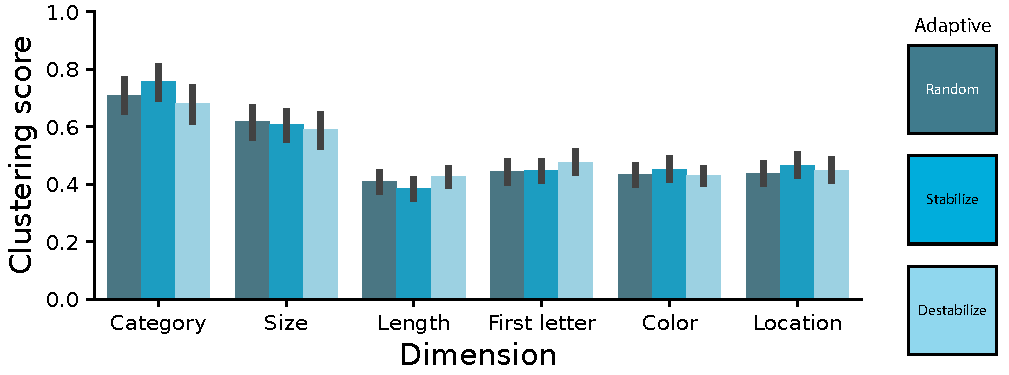
\includegraphics[width=\textwidth]{figures/fingerprints_adaptive}
    
    \caption{\textbf{Memory ``fingerprints.'' (adaptive conditions).}
    The across-participant distributions of clustering scores for each feature
    type ($x$-coordinate) are displayed for each experimental condition
    (color), separately for order manipulation (early, top) and randomly
    ordered (late, bottom) lists.}
        \label{fig:fingerprints-adaptive}
\end{figure}

\begin{sidewaysfigure}
    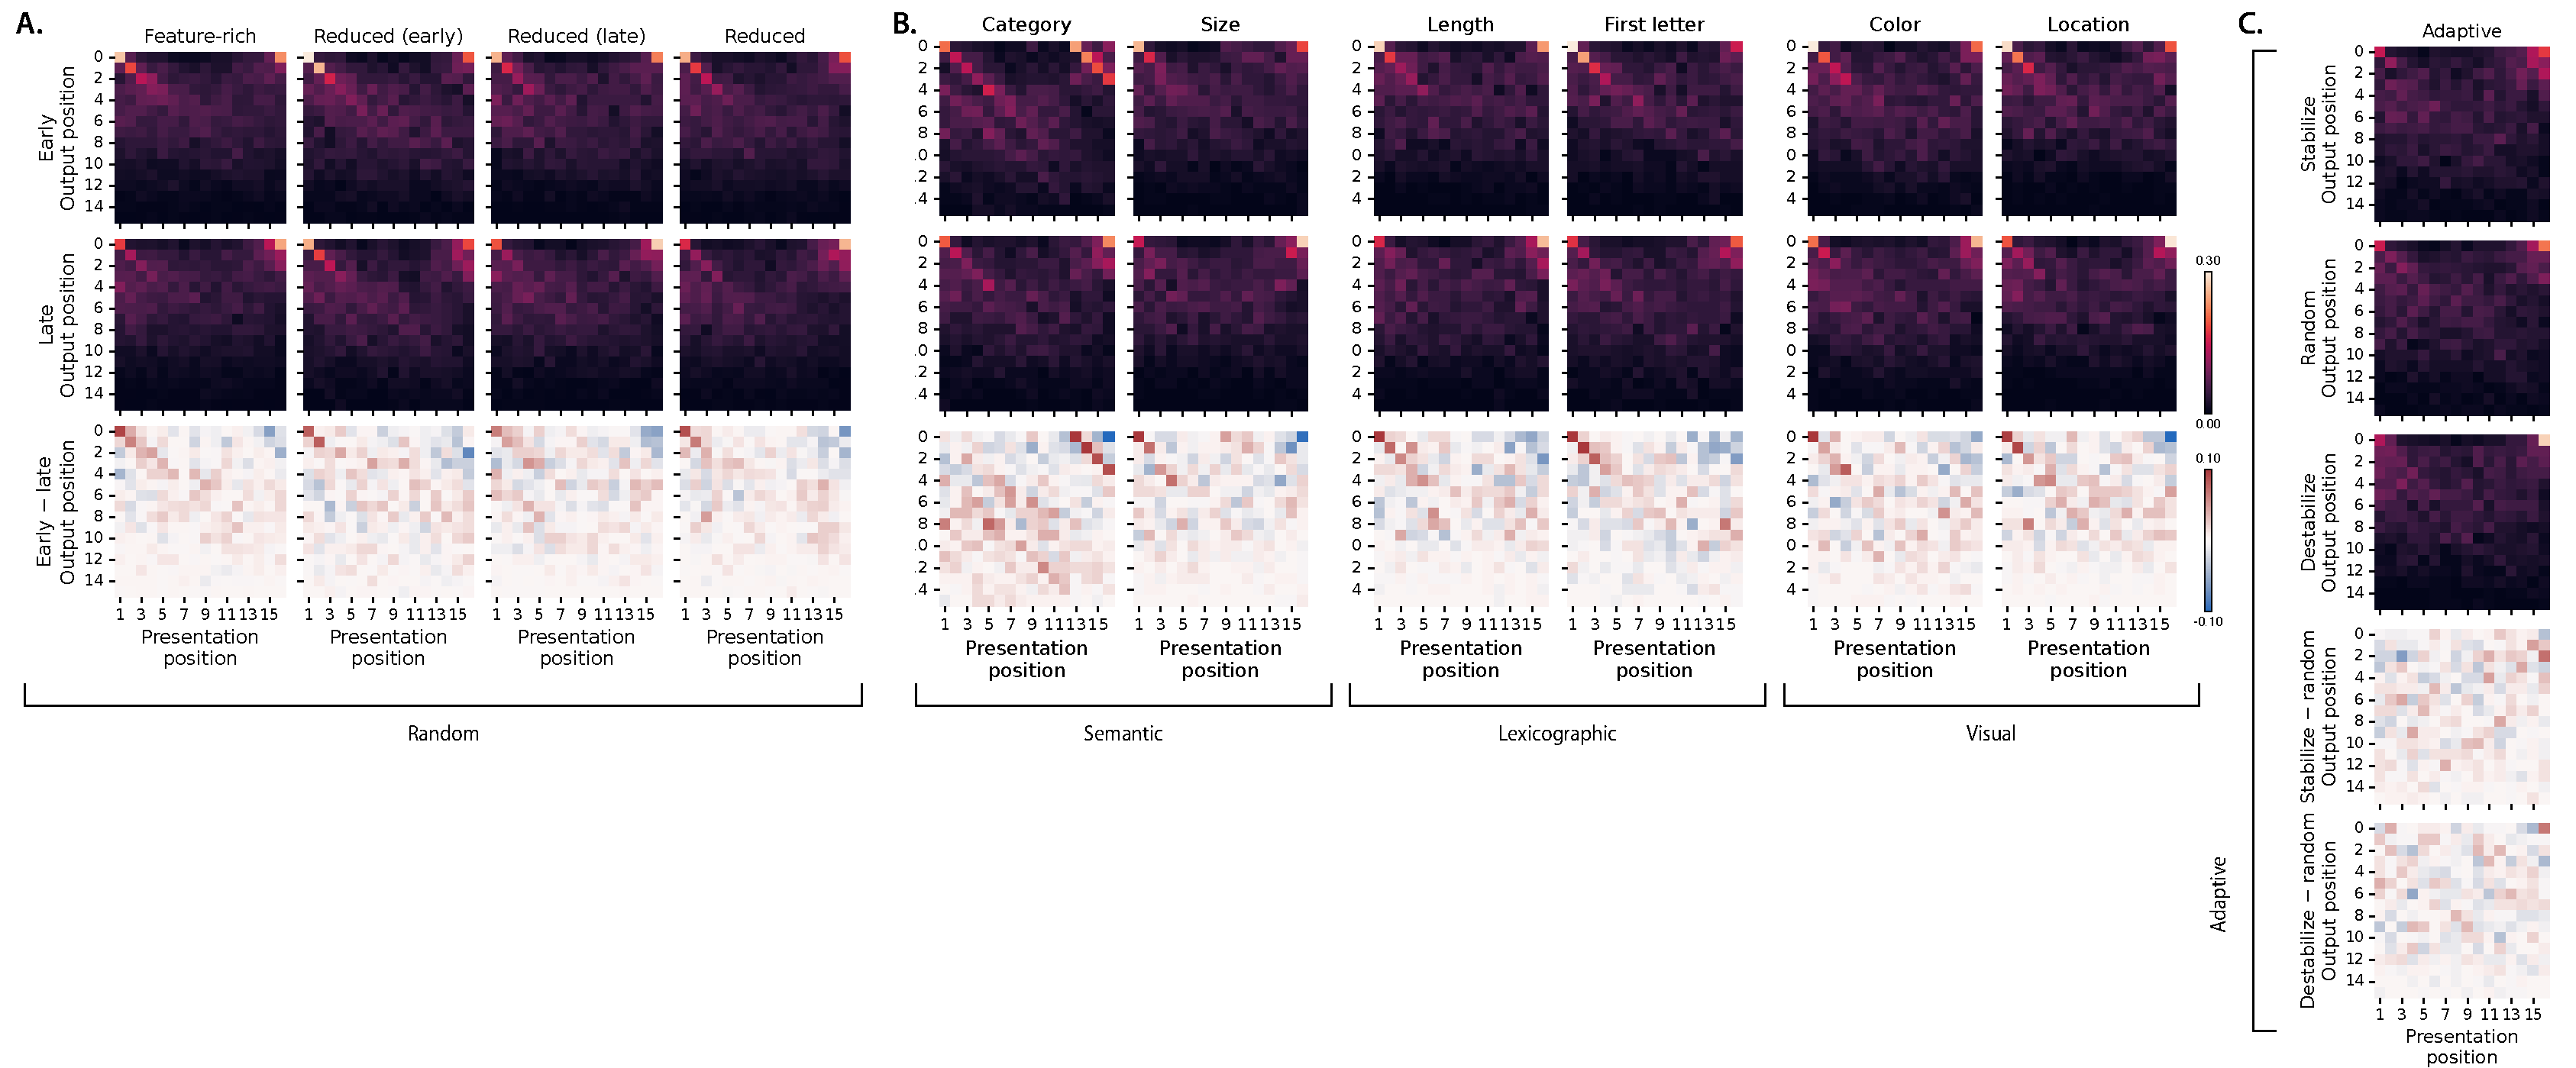
\includegraphics[width=\textwidth]{figures/pnr_matrices}

    \caption{\textbf{Probability of $n$\textsuperscript{th} recall matrices.}  Each sub-panel displays
    the average probability of recalling the given word (Presentation position, $x$-coordinate)
    at the given output position ($y$-coordinate); color denotes the probability.  \textbf{A. Random conditions.}  The top rows
    display data from early (order manipulation) lists, the middle rows display data from late (randomly ordered)
    lists, and the bottom rows display the differences between the matrices in the top and middle rows.  Panel columns denote experimental conditions.
    \textbf{B. Order manipulation conditions.}  The matrices are displayed in the same format as those in Panel A.
    Panel columns are organized by feature type (semantic, lexicographic, or visual).  \textbf{C. Adaptive conditions.}
    The sub-panels are displayed in the same formats as Panels A and B, but here the matrices
    and contrasts (indicated in $y$-axis labels) reflect different list manipulation conditions.}

    \label{fig:pnr}
\end{sidewaysfigure}

\newpage
\renewcommand{\refname}{Supplementary references}
\bibliographystyle{apa}
\bibliography{CDL-bibliography/cdl}



\end{document}
